\chapter{Legged Robotics}
\subsection{Introduction}
Most of surface lands are inaccessible to wheeled robots, leading to the necessity of alternative motion systems. One of these are the so-called \textit{legged} robots, whose structure often imitates animals and/or insects. 
\subsection{Taxonomy}
There are a great many types of legged robots, classified by:
\begin{itemize}
    \item Stability of gait:
    \begin{itemize}
        \item \textit{Statically stable gait}(fig: \ref{fig:statically_stable_robot}): the robot control its locomotion such that the vertical projection of the center of gravity is always contained within the support polygon. Generally speaking, these robots are slow.
        \item \textit{Dinamically stable gait}(fig: \ref{fig:dinamically_stable_robot}): the robot is not statically balanced during the locomotion, the support polygon has degenerated to a point or a line.
    \end{itemize}
    \begin{figure}[htbp!]
        \begin{minipage}{0.5\textwidth}
            \centering
            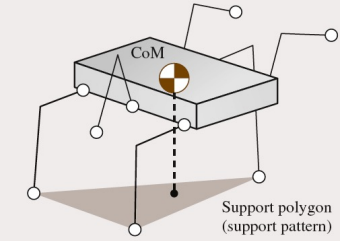
\includegraphics[width=0.5\linewidth]{Images/statically_stable_robot.png}
            \caption{Support Poligon for\\ statically stable robot.} 
            \label{fig:statically_stable_robot}
        \end{minipage}\hfill 
        \begin{minipage}{0.5\textwidth}
            \centering
            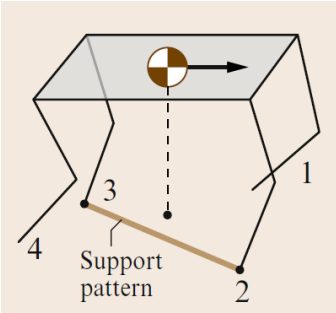
\includegraphics[width=0.5\linewidth]{Images/dinamic_stable_gait.png}
            \caption{Support Poligon for\\ dinamically stable robot.}
            \label{fig:dinamically_stable_robot}
        \end{minipage}
    \end{figure}
    \item Number of legs: monopod, bipod, etc.
    \item Type of leg articulation:
    \begin{figure}[htbp!]
        \begin{minipage}{0.7\textwidth}
            Mainly composed by a rotating and a linear actuator. It's the simplest structure possible, which however leads to low adaptability to uneven terrains.
        \end{minipage}\hfill 
        \begin{minipage}{0.3\textwidth}
            \centering
            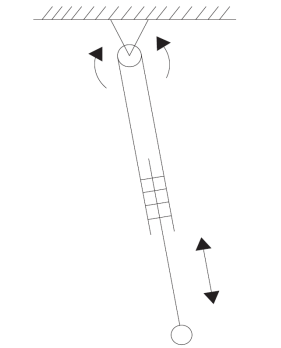
\includegraphics[width=0.5\linewidth]{Images/prismatic_leg.png}
            \caption{Prismatic Leg.}
            \label{fig:prismatic_leg}
        \end{minipage}\vfill 
        \begin{minipage}{0.4\textwidth}
            \centering
            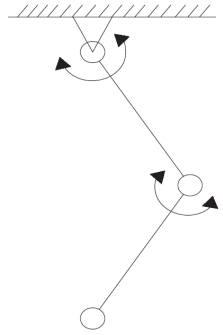
\includegraphics[width=0.4\linewidth]{Images/articulated_leg.png}
            \caption{\\Articulated Leg.}
            \label{fig:articulated_leg}
        \end{minipage}\hfill
        \begin{minipage}{0.6\textwidth}
            Compared with prismatic legs, the articulated leg uses a rotating joint instead of a linear prismatic joint to achieve leg length control. It is usually used in robot with four and more legs, with the addition of a perpendicular joint that enables the lateral motion.
        \end{minipage}\vfill 
        \begin{minipage}{0.7\textwidth}
            The extension of the articulated legs with at least one more rotating joint. Usually used in biped robots, with the addition of other joints along the different axes that are useful to improve the stability.
        \end{minipage}\hfill
        \begin{minipage}{0.3\textwidth}
            \centering
            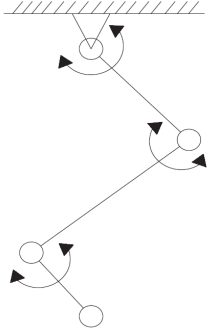
\includegraphics[width=0.5\linewidth]{Images/redundant_articulated_leg.png}
            \caption{\\Redundant\\ Articulated Leg.}
            \label{fig:redundant_articulated_leg}
        \end{minipage}
    \end{figure}
\end{itemize}

For the specific instance of quadruped robots, there is also another distinction based on the structure of the leg kinematic chain.
\begin{itemize}
    \item Forward elbow, backward knee: the optimal configuration, giving better locomotion stability and little impact force between foot and ground.
    \item Forward knee, backward elbow.
    \item Knees.
    \item Elbows.
\end{itemize}
Control also represents a challenge, since there is a need to maximize torque, bandwidth, and power meanwhile minimizing friction, inertia, and mass loss. New actuators designs are also needed to reduce the effects of the high mechanical impedance resulting from the impact with the ground, such as \textit{Series Elastic Actuators} or \textit{Proprioceptive Actuators}. Finally, navigation causes the need of a large amount of onboard sensors, many of which highly complex and costly (such as LIDARs).
\subsection{Dynamic Model}
A legged robot's configuration is fully described by the coordinates of its \textit{floating base} (the body) and the configurations of its legs.
\begin{figure}[htbp!]
    \begin{minipage}{0.5\textwidth}
        \centering
        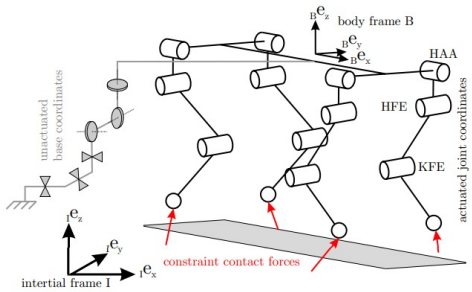
\includegraphics[width=1\linewidth]{Images/floating_base_scheme.png}
        \caption{Legged robot structure.}
        \label{fig:floating_base_scheme}
    \end{minipage}\hfill
    \begin{minipage}{0.5\textwidth}
        The former is accomplished by defining the vectors of  $p_b\in\mathbb{R}^3,R_b\in SO(3)$ describing position and orientation of the body frame with respect to the world frame, as usual; the latter, is obtained by defining the generalized coordinate vector $q=[q_b^T, q_j^T]^T\in\mathbb{R}^{n_b+n_j}$, of which the dimension is dependent on the choice of rotation parameterization.
    \end{minipage} 
\end{figure}\\
Usually, if a minimal representation is used, $q_b=[p_b^T,\eta_b^T]^T\in\mathbb{R}^6$, where $\eta_b$ are the Euler angles. Once a description of the structure is obtained, it is now possible to describe the robot's motion. A distinction between \textit{stance feet}, the ones touching the ground, and \textit{swing feet}, the ones who don't, is needed; then, the contacts are modeled as kinematic constraints imposed on the stance feet.
\begin{figure}[htbp!]
    \begin{minipage}{0.5\textwidth}
        \centering
        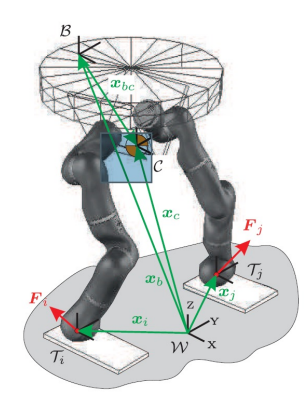
\includegraphics[width=0.75\linewidth]{Images/stance feet.png}
        \caption{Stance feet.}
        \label{fig:stance_feet}
    \end{minipage}\hfill
    \begin{minipage}{0.5\textwidth}
        \begin{definition}
            (\textit{Contact point constraint}): During robot's operation, for the $i$-th stance foot, it must hold the following \textit{non-slipping constraint}:
            \begin{gather}
                p_i=const,\quad
                \dot{p}_i=0_3,\quad
                \ddot{p}_i=0_3
            \end{gather}
            Which can be expressed a \textit{contact Jacobian} mapping the robot's generalized velocity vector into the stance feet generalized velocity vector:
            \begin{equation}\label{contact_jacobian}
                J_{T_i}=
                \begin{bmatrix}
                    \begin{bmatrix}
                        I_3 & S(p_{bi}) \\
                        0_{3\times 3} & I_{3}
                    \end{bmatrix} & J_i       
                \end{bmatrix}\in\mathbb{R}^{6\times(n_b+n_j)}
            \end{equation}
            Where $p_{bi}=p_b-p_i,J_i=\partial(r_i-q_b)/\partial q_j\in\mathbb{R}^{6\times n_j}$ and $r_i$ is the vector of the $i$-th stance foot's pose.
        \end{definition}
    \end{minipage} 
\end{figure}\\
In the particular case of a quadruped robot, the pose of the foot coincides with its position, so that the contact Jacobian becomes:
\begin{gather}\label{point_contact_Jacobian_for_quadruped_robot}
    J_{T_i}=
    \begin{bmatrix}
        I_3 & S(p_{bi}) & J_{p,i}
    \end{bmatrix}\in\mathbb{R}^{3\times (n_b+n_j)}
\end{gather}
Where $J_{p,i}$ is composed of only the first three rows of $J_i$. For an $n_{st}$ stance feet robot, the contact Jacobians are stacked into a single Jacobian:
\begin{gather}\label{total_contact_jacobian}
    J_{st}=
    \begin{bmatrix}
        J_{st,b} & J_{st,i}
    \end{bmatrix}\in\mathbb{R}^{3n_{st}\times (n_b+n_j)}
\end{gather}
Obviously, the contact points cause \textit{Ground Reaction Forces}, which push against the robot legs. It is only because of these forces that a legged robot is able to move. In turn, GRFs cause friction (which is helpful in avoiding slipping) and this has to be taken into account in the model. The most basic friction model is the \textit{Coulomb Friction Model}, which states that.
\begin{definition}
    \textit{(Coulomb Friction Model)}: Define $f_x,f_y,f_z$ as the projections of the GRFs on the axes associated to the single point contact $C_i$. Then, the friction caused by the GRFs is given as:
    \begin{equation}\label{Coulomb_Friction_Model}
        \sqrt{f_x^2+f_y^2}=\mu f_z
    \end{equation}
    Where $\mu$ is the friction coefficient.
\end{definition}
Notice that the model is, geometrically speaking, a cone (from which the alternative name \textit{friction cone model}) and is nonlinear. In order to ease the real-time computation, a linear approximation is implemented by inscribing or circumscribing a pyramid shape against the cone. In particular, the stricter version (inscribing) is used and is defined as the model:
\begin{definition}
    \textit{(Inscribed Pyramidal Friction Model):}
    \begin{gather}\label{inscribed_pyramid_friction}
        |f_x|\leq \frac{\sqrt{2}}{2}\mu f_z\\
        |f_y|\leq \frac{\sqrt{2}}{2}\mu f_z
    \end{gather}
\end{definition}
\begin{figure}[h!]
    \centering
    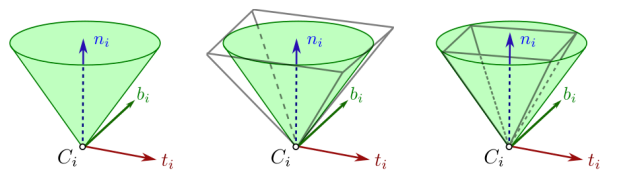
\includegraphics[width=0.75\linewidth]{Images/pyramid_friction_model.png}
    \caption{Pyramid Friction Model scheme.}
\end{figure}
Finally, the dynamic of a floating base robot can be written.
\begin{definition}
    \textit{Floating Base Robot Dynamics}:
    \begin{equation}\label{legged_robot_dynamic_model}
        M(q)\dot{v}+Cv+g=S^{T}\tau+J_{st}^{T}f_{gr}+J^{T}f_{ext}
    \end{equation}
    Where:
    \begin{itemize}
        \item $M(q)\in\mathbb{R}^{(n_b+n_j)\times(n_b+n_j)}$ is the inertia matrix.
        \item $C\in\mathbb{R}^{(n_b+n_j)\times(n_b+n_j)}$ is the Coriolis term.
        \item $g\in\mathbb{R}^{n_b+n_j}$ is the gravitational term.
        \item $S=[O_{n_j\times6},I_{n_j}]$ is the \textit{torque distribution matrix} selecting the actuated joints.
        \item $f_{gr}\in\mathbb{R}^{3n_{st}}$ is the vector of ground reaction forces (GRFs).
        \item $\tau\in\mathbb{R}^{n_j}$ is the vector of joint actuation forces.
        \item $J$ is the staked matrix of the feet Jacobians.
        \item $f_{ext}$ is the vector containing the net forces at the legs' tips accounting for unmodelled dynamics and disturbances.
    \end{itemize}
\end{definition}
\subsection{Constrained Consistent Dynamics}
A legged robot can be controlled by an inverse dynamics approach; however, the dynamic model in eq:\ref{legged_robot_dynamic_model} is not sufficient, since it does not take into account the contact constraints. A \textit{constrained consistent dynamic} model can be obtained starting from the formulation of an appropriate projection operator $N_c$, such that it takes directly into account the contact constraints. 
\begin{definition}
    \textit{(Constrained Consistent Dynamics model):} Define the model:
    \begin{equation}\label{constrained_consistent_dynamic_model}
        N_c\left(M\dot{v}+Cv+g-J^{T}f_{ext}\right)=N_cS^{T}\tau
    \end{equation}
    Where the projection operator $N_c$ is defined as:
    \begin{equation}\label{legged_robotics_dynamically_consistent_projection_operator}
        N_c=I_{n_{st}}-\left[M^{-1}J_{st}^{T}\left(J_{st}M^{-1}J_{st}^{T}\right)\right]=I_{n_{st}}-J_{st}^{*}J_{st}
    \end{equation}
    It defines a generalized space of motion with no acceleration or force couplings effects on the stance legs. This dynamics can be inverted to follow a desired acceleration, applying the input:
    \begin{equation}\label{legged_robot_inverted_dynamics_input}
        \tau^*=\left(N_cS^T\right)^*N_c\left(M\dot{v}+Cv+g-J^{T}f_{ext}\right)
    \end{equation}
\end{definition}
The input can also take into account another term, which changes the torque distributions on the legs.
\begin{equation}\label{legged_robot_inverted_dynamics_augmented_input}
    \tau^*=\left(N_cS^T\right)^*N_c\left[M\dot{v}_d+Cv+g\right]+\mathcal{N}\left(N_cS^T\right)\tau_0^*
\end{equation}
Notice that if Rank$(J_{st,b})=6$ the body position is fully controllable by the joints; however, with a two point contact (such as for a quadruped robot), the rank is not full and the system is not fully controllable.
\section{Balancing}
\subsection{Centroidal Dynamics}
Generally speaking, the position of the robot's center of mass could not coincide with the body frame's origin. To solve this, a simple coordinate transformation can be carried out by defining a coordinate system at the CoM position (with respect to the body frame)  $p_c\in\mathbb{R}^{3\times1}$ and the same orientation as the body frame. Then, the CoM's velocity relative to the body frame is:
\begin{gather}
    \begin{bmatrix}
        \dot{p}_c \\ \omega_c \\ \dot{q}_j
    \end{bmatrix}=
    \begin{bmatrix}
        I_3 & -S(p_{bc}) & J_{bc}\\
        0_3 & I_3 & 0_3\\
        0_3 & 0_3 & I_{n_j}
    \end{bmatrix}
    \begin{bmatrix}
        \dot{p}_b \\ \omega_b \\ \dot{q}_j
    \end{bmatrix}=\\
    =\bar{T}v_b
\end{gather}
Applying this transformation to the robot's model as in eq:\ref{legged_robot_dynamic_model} leads to the so-called \textit{Centroidal Dynamics Model}.
\begin{definition}
    \textit{(Centroidal Dynamics Model)}: Define the transformation:
    \begin{equation}\label{legged_CoM_coord_trans}
        \bar{T}=
        \begin{bmatrix}
            I_3 & -S(p_{bc}) & J_{bc}\\
            0_3 & I_3 & 0_3\\
            0_3 & 0_3 & I_{n_j}
        \end{bmatrix}
    \end{equation}
    As the mapping which expresses the robot's center of mass velocities with respect to the body frame velocities. Then, the dynamic model of a legged robot expressed with respect to the Center of Mass position is:
    \begin{equation}\label{legged_Centroidal_Dynamics_Model}
        \begin{bmatrix}
            mI_3 & 0_3 & 0_{3\times n_j}\\
            0_3 & M_{11} & 0_{3\times n_j}\\
            0_{n_j\times 3} & 0_{n_j\times 3} & M_{22}
        \end{bmatrix}
        \dot{v}_c+
        \begin{bmatrix}
            0_3\\
            \bar{C}_1\\
            \bar{C}_2
        \end{bmatrix}v_c+
        \begin{bmatrix}
            mg_0\\ 0_3 \\ 0_{n_j}
        \end{bmatrix}=S^{T}\tau+
        \begin{bmatrix}
            \bar{J}_{st,c}^{T}\\
            \bar{J}_{st,j}^{T}f_{gr}
        \end{bmatrix}+
        \begin{bmatrix}
            \bar{J}_{c}^{T}\\ \bar{J}_{j}^{T}f_{ext}
        \end{bmatrix}
    \end{equation}
    Where:
    \begin{multicols}{2}
        \begin{itemize}
            \item $m$ is the robot's mass.
            \item $\bar{M}=\bar{T}^{-T}M\bar{T}^{-1}$.
            \item $\bar{C}=\bar{T}^{-T}C\bar{T}^{-1}+\bar{T}^{-T}M\frac{d\bar{T}^{-1}}{dt}$.
            \item $\bar{J}_{st}=J_{st}\bar{T}^{-1}$.
            \item $\bar{J}=J\bar{T}^{-1}$.
            \item $v_c=[\dot{p}_c^T,\omega_c^T,\dot{q}_j^T]^T$.
        \end{itemize}
    \end{multicols}
\end{definition}
Notice that if the angular motion is slow and the legs' masses are negligible when compared to the body's mass, then the $\bar{C}_1$ term is negligible. Also, if external disturbances are perfectly compensated for, then the model completely decouples the linear and angular CoM's dynamics; this implies that an inverse dynamics approach can be used to extract the joints' dynamics directly from the model's last rows.
\begin{definition}\label{legged_CoM_inverse_dynamics}
    \textit{Inverse Dynamics Control for Centroidal Dynamics}: In the model eq:\ref{legged_Centroidal_Dynamics_Model}, assume that all external disturbances are compensated for. Then, an \textit{inverse dynamics} approach can be implemented to control the robot. The input law is:
    \begin{equation}\label{legged_CoM_inverse_dynamics_input}
        \tau^*=M_{22}\ddot{q}_j^*+\bar{C}_2v-\bar{J}_{st,j}f^*_{gr}
    \end{equation}
    Where $\ddot{q}_j^*$ and $f_{gr}^*$ are the desired joints' acceleration and ground reaction forces, respectively.
\end{definition}
\subsection{Complementarity Constraints}
It is always appropriate to remark that a legged robot can only move when there is contact with the ground; this is such an important concept that it has to be included in the model; this is done by adding the so-called the \textit{Complementarity Constraints}, which account for:
\begin{itemize}
    \item The ground can only push, not pull, on the robot.
    \item The feet can only impact on the ground, not penetrate it.
    \item A reaction force acts on the $i$-th stance foot if and only if there is contact to the ground: the distance between the contact point of the foot and the ground must be zero.
\end{itemize}
Then, the centroidal dynamics model in eq:\ref{legged_Centroidal_Dynamics_Model} is augmented.
\begin{definition}\label{legged_robot_compl_const_model}
    \textit{Augmented legged robot model with Complementarity Constraints}: Consider the Centroidal Dynamics model in eq:\ref{legged_Centroidal_Dynamics_Model}; then, in the case of contact with the ground, the following augmented model holds:
    \begin{gather}\label{legged_robot_compl_const_model_eq}
        \bar{M}(q_c)\bar{v}_c+\bar{C}(q_c,v_c)v_c+\bar{g}(q_c)=S^{T}\tau+\nabla F(q_c)\lambda_n+P_t(q_c,v_c)\\
        \lambda^{T}_nF(q_c)=0\\
        \lambda_n\geq0\\
        F(q_c)\geq0
    \end{gather}
    Where:
    \begin{multicols}{2}
        \begin{itemize}
            \item $F(q_c)$ represents the distance between the $m$ possible contact points on the feet from the ground.
            \item $\lambda_n$ is the vector of ground reaction forces at the $m$ contact points.
            \item $P_t(q_c,v_c)$ is the vector of GRF's tangential components.
        \end{itemize}
    \end{multicols}
\end{definition}
\subsection{Introduction to stability conditions}
In the context of legged robotics it is most important to know if and when the robot could fall. There are may ways to answer this question, but before addressing them, it is necessary to define what the \textit{Center of Pressure} or \textit{Zero Moment Point} is.\\
From rigid-body dynamics, recall that the center of mass dynamics is neatly described by:
\begin{gather*}
    m\ddot{p}_c=mg_0+\sum_{i=1}^{n_{st}}f_{gr,i}\\
    I\dot{\omega}=\sum_{i=1}^{n_{st}}p_{ci}\times f_{gr,i}
\end{gather*}
Where $p_{ci}$ is the distance between the CoM and the $i$-th contact point. Assume that each contact point has zero $\hat{z}$-component, so that $p_z^{(i)}=0$. To obtain the definition of the \textit{Center of Pressure}, start by balancing the torques applied to the CoM:
\begin{gather*}
    mp_c\times(\ddot{p}_c-g_0)+\dot{L}=\sum_{i=1}^{n_{st}}p_i\times f_{gr,i}
\end{gather*}
Then, divide this by the third linear dynamic equation:
\begin{gather*}
    \frac{mp_c\times(\ddot{p}_c-g_0)+\dot{L}}{m(\ddot{p}_c^z-g_0^z)}=\frac{\sum_{i=1}^{n_{st}}p_i\times f_{gr,i}}{\sum_{i=1}^{n_{st}}f_{gr,i}^{z}}\\
    \text{Since $p_{i}^z=0$ the $x,y$ coordinates are:}\\
    p_c^{x,y}-\frac{p_z^c}{\ddot{p}_c^z-g_0^z}\left(\ddot{p}_c^{x,y}-g_0^{x,y}\right)+\frac{s\dot{L}^{x,y}}{m\left(\ddot{p}_c^z-g_0^z\right)}=\frac{\sum_{i=1}^{n_{st}}f_{gr,i}^{z}p_{i}^{x,y}}{\sum_{i=1}^{n_{st}}f_{gr,i}^{z}},\\
    S=\begin{bmatrix}
        0 & -1 \\ 1 & 0
    \end{bmatrix}\in SO(2)
\end{gather*}
\begin{definition}\label{legged_robotics_Center_of_pressure}
    \textit{Center of Pressure}: A legged robot's \textit{center of pressure} is defined to be the point:
    \begin{equation}\label{legged_robotics_Center_of_pressure_equation}
        p_z=\frac{\sum_{i=1}^{n_{st}}f_{gr,i}^{z}p_{i}^{x,y}}{\sum_{i=1}^{n_{st}}f_{gr,i}^{z}}
    \end{equation}
    For which:
    \begin{equation*}
        \sum_{i=1}^{n_{st}}f_{gr,i}^{z}(p_z^{x,y}-p_{i}^{x,y})=0
    \end{equation*}
    Meaning that the  GRFs' horizontal momenta, computed with respect to the CoP, are null; this is why the CoP is also called \textit{Zero Moment Point}(ZMP).\\
    Since the GRFs are unilateral, $f_{gr,i}^{z}\geq0$, the CoP is bound to be contained in the convex hull of the point contacts. This is expressed by the \textit{Ordinary Differential Inclusion}:
    \begin{equation}\label{legged_robotics_CoP_ODI}
        p_c^{x,y}-\frac{p_z^c}{\ddot{p}_c^z-g_0^z}(\ddot{p}_c^{x,y}-g_0^{x,y})+\frac{1}{m(\ddot{p}_c^z-g_0^z)}S\dot{L}^{x,y}\in \text{conv}\{p_{i}^{x,y}\}
    \end{equation}
\end{definition}
Notice that the horizontal acceleration of the CoM is the result of a force pushing the CoM away from the CoP; this is an intrinsically unstable dynamics. \\
A legged robot's stability can be analyzed by considering:
\begin{itemize}
    \item \textit{Fixed Points}: they represent the static postures in which the robot can safely stand still.
    \item \textit{Limit Cycles}: they provide an instrument to describe walking and runnnig motion.
    \item \textit{Viability}: a concept of controlled invariance, which analyses the set of states from which the robot is able to avoid to fall.
    \item \textit{Controllability}: it provides a slightly restricted notion of viability, analysing the set of states from which the robot is capable of returning to a particular fixed point or limit cycle.
\end{itemize}
It is also important to understand which kind of stability can be achieved:
\begin{itemize}
    \item \textit{Robust Stability}: it examines the properties of the system considering worst-case (bounded) disturbances.
    \item \textit{Stochastic Stability}: it makes use of tools to investigate the probability of falling down.
    \item \textit{Input-Output Stability}: it treats a particular disturbance as an input, a performance criteria as output, and attempts to compute a relative gain or sensitivity of the robot performance due to this input.
    \textit{Stability Margins}: in practice control designers often settle for the system staying comfortably away from the boundaries of deterministic stability.
\end{itemize}
\subsubsection{Fixed Points}
For a robot to stand still it must hold $\ddot{p}_c=\dot{L}=0$, so that the ODI eq:\ref{legged_robotics_CoP_ODI} can be written as:
\begin{equation*}
    p_c^{x,y}-\frac{p_c^z}{g_0^z}g_0^{x,y}=p_{z}^{x,y}\in \text{conv}\{p_i^{x,y}\}
\end{equation*}
This necessary condition states that the CoM must project on the ground along the gravity vector inside the convex hull of the contact points of the stance legs; this convex hull is defined as the \textit{support polygon}. Once a fixed point has been found, the usual techniques of nonlinear stability analysis can be used to examine its stability. For example, linearization of the robot's model can give local results about it.
\subsubsection{Limit Cycles}
Robots with more actuators typically have an abundance of periodic solutions and planning techniques can be used to find those that, for instance, minimize a quantity of interest such as the cost of transport or a measure of open-loop stability. Under mild conditions, a sufficient criteria for establishing orbital stability is establishing fixed-point stability of a Poincaré map, as is known from nonlinear stability theory. However, during a locomotion task in a nontrivial environment, the motions could be aperiodic; in those instances, a \textit{moving} Poincaré section can be used. It is important to notice that more often than not these analyses are conducted numerically.
\section{Control of Legged Robots}
Control of legged robots is executed by decoupling the planning part from the purely control part. To do so, a \textit{whole-body} controller is implemented.
\begin{figure}[h!]
    \centering
    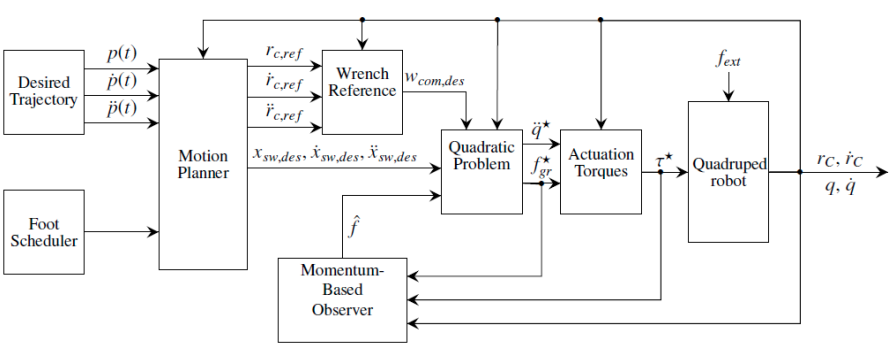
\includegraphics[width=0.75\linewidth]{Images/legged_robots_whole_body_controller.png}
    \caption{\textit{Whole-Body} Controller.}
    \label{fig:legged_whole_body_controller}
\end{figure}\\
This controller computes the desired joint accelerations $\ddot{q}_j^*$ and GRFs $f_{gr}^*$. Its inputs are:
\begin{itemize}
    \item A desired CoM's trajectory.
    \item The foot schedule, which is a function of the robot's gait, such as \textit{Trot} (cross legs move), \textit{Pace} (lateral legs work in coordination), \textit{Bound} (front and rear legs work in pair).
\end{itemize}
Then, a wrench-reference is computed and passed onto a Quadratic Solver, which solves a quadratic constrained problem. The constraints take care of dynamic consistency, non-sliding contacts, torque limits and swing legs tasks. Notice also the presence of a momentum-basd observer, which computes the external forces acting on the robot to compensate for them in the control. Let us look at the components more closely now.
\subsection{Motion Planner}
The motion planner takes as input a desired trajectory for the CoM and a foot schedule, giving as output the appropriate references; these are, generally speaking, regular curves, but due to numerical errors a drift can appear between the torso and feet movements, which is corrected at each planning step by the motion planner. The complete motion is divided into a \textit{Stance Phase} and a \textit{Swing Phase} by the foot-scheduler; then, desired path is composed by splines such that:
\begin{itemize}
    \item The initial state $p(0),\dot{p}(0),\ddot{p}(0)$ coincide with the center of the initial support polygon an the initial velocity and acceleration.
    \item The final state $p(t_f),\dot{p}(t_f),\ddot{p}(t_f)$ is set to be at the center of the polygon defined by the planned footholds, which is the polygon that would support the robot if it was to stop and stand at the end of the support polygon sequence.
\end{itemize}
Given the swing-phase duration $T_{sw}$ and the maximum step length, the motion planner computes a sequence of footholds.\\
During the stance-phase: the legs are all in contact with the ground, ensuring an intrinsic balance; the CoM reference $r_{c,ref}, \dot{r}_{c,ref}, \ddot{r}_{c,ref}$ can be computed as a 3-rd order spline that tracks the desired trajectory.\\
During the swing-phase: since at least one leg is swinging, both the CoM's trajectory and the swing feet motion have to be planned. Considering the reference $r_{c,ref}=[p_{c,ref}^{T},\eta_{c,ref}^{T}]^{T}$, the motion CoM's coordinates can be described by the $i$-th spline as:
\begin{gather*}
    p_{c,ref}^{(x)}=\alpha_{i3,x}t^{3}+\alpha_{i2,x}t^2+\alpha_{i1,x}t+\alpha_{i0,x}\\
    p_{c,ref}^{(y)}=\alpha_{i3,y}t^{3}+\alpha_{i2,y}t^2+\alpha_{i1,y}t+\alpha_{i0,y}\\
    p_{c,ref}^{(z)}=\alpha_{i3,z}t^{3}+\alpha_{i2,z}t^2+\alpha_{i1,z}t+\alpha_{i0,z}
\end{gather*}
Which can be restated as:
\begin{gather}
    \lambda(t)=
    \begin{bmatrix}
        t^3 & t^2 & t & 1
    \end{bmatrix},\\
    \alpha_{ik}=
    \begin{bmatrix}
        \alpha_{ik,x} & \alpha_{ik,y} & \alpha_{ik,z}    
    \end{bmatrix}^{T},\\
    \begin{bmatrix}
        \alpha_{i3} & \alpha_{i2} & \alpha_{i1} & \alpha_{i0}
    \end{bmatrix},\\
    T=
    \begin{bmatrix}
        \lambda(t) & 0 & 0\\
        0 & \lambda(t) & 0\\
        0 & 0 & \lambda(t)
    \end{bmatrix}, \\
    p_{c,ref}=T\alpha_i,\\
    \dot{p}_{c,ref}=\dot{T}\alpha_i,\\
    \ddot{p}_{c,ref}=\ddot{T}\alpha_i
\end{gather}
The motion planning algorithm is then formulated as a constrained nonlinear optimization problem which minimizes a generic cost function, with the spline stacked vector $\alpha_i$ as optimization variables. To ensure splines continuity, the following junction constraint is added:
\begin{gather}
    \begin{bmatrix}
        \lambda(t_{f_k})^{T} & -\lambda(0)^{T}\\
        \dot{\lambda}(t_{f_k})^{T} & -\dot{\lambda}(0)^{T}
    \end{bmatrix}
    \begin{bmatrix}
        \alpha_{k}^{x}\\
        \alpha_{k+1}^{x}
    \end{bmatrix}=0
\end{gather}
Where $t_{f_k}$ is the duration of spline $s_k$. Some constraints are also added to ensure stability, by constraining the ZMP (see definition n.\ref{legged_robotics_Center_of_pressure}) to stay inside the robot's support polygon. In particular, starting from the measured feet configuration, the motion plan is called and, using the planned feet positions, a sequence of support polygons and their duration is computed by using the contact schedule. 
\begin{figure}[htpb!]
    \centering
    \begin{minipage}{0.7\textwidth}
        \centering
        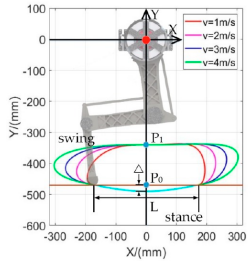
\includegraphics[width=0.7\linewidth]{Images/legged_swing_feet.png}
        \caption{Swing Feet splines.}
    \end{minipage}\hfill
    \begin{minipage}{0.3\textwidth}
        This can be achieved by imposing the constraint:
        \begin{gather*}
            ap_z^x+bp_z^y+c\geq 0
        \end{gather*}
        Where $a,b,c$ are the coefficients of the line passin through the vertices of an edge of the support polygon.\\
        Finally, the reference for the swing feet is computed using two splines, the former to lift the foot, the latter to lower it.
    \end{minipage}
\end{figure}
\subsection{Momentum Based Observer}
External forces are estimated to compensate for them inside the controller; in order to take into account the disturbances acting on both stance and swing legs, the observer considers the momentum of all the legs, given by:
\begin{equation}
    \dot{\rho}=\bar{C}_{2}^{T}\dot{q}_{j}+\bar{J}_{st,j}^{T}f_{gr}+\tau+\bar{J}_{j}^{T}f_{ext}
\end{equation}
By defining:
\begin{itemize}
    \item $\hat{F}=\bar{J}_{j}^{T}\in\mathbb{R}^{n_j}$, which represents the estimated joint torques corresponding to the resultant force at the legs' tips.
    \item $F_{ext}=\bar{J}_{j}^{T}f_{ext}\in\mathbb{R}^{n_j}$, which represents the effect at the joint torques of the resultant force at the legs' tips.
\end{itemize}
The estimator can be designed to achieve a linear relationship between the estimated external forces and the real ones in the Laplace domain as:
\begin{definition}\label{legged_estimator}
    \textit{Legged Robot Momentum-Based Observer}: The Momentum-Based Observer used in the Whole-Body controller is designed as:
    \begin{gather}\label{legged_estimator_eq}
        \hat{F}=G(s)F_{ext}\\
        \alpha(t)=\bar{C}_{2}^{T}\dot{q}_{j}+\tau+\bar{J}_{st,j}^{T}f_{gr}\\
        \gamma_1=K_1\left[\rho(t)-\int_{0}^{t}\left(\hat{F}(\sigma)+\alpha(\sigma)\right)d\sigma\right]\\
        \gamma_i=K_i\int_{0}^{t}{\left(-\hat{F}(\sigma)+\gamma_{i-1}(\sigma)\right)d\sigma}, \quad i=2,\dots,r
    \end{gather}
    Where:
    \begin{itemize}
        \item $r$ is the desired estimator's degree.
        \item $\hat{F}=\gamma_r$.
        \item $K_i\in\mathbb{R}^{n_j\times n_j}$ are positive definite matrices.
    \end{itemize}
\end{definition}
\subsection{Quadratic Problem}
The desired acceleration and the desired ground reaction forces are obtained through a quadratic problem, formally defined as:
\begin{definition}\label{legged_quadratic_problem}
    \textit{(Legged Robot's Quadratic Problem for Motion Planning)}: The QP used in the Whole-Body Controller is formally defined as:
    \begin{gather*}
        \zeta=
        \begin{bmatrix}
            \ddot{r}_{c}^{T} & \ddot{q}_{j}^{T} & f_{gr}^{T}
        \end{bmatrix}\in\mathbb{R}^{n_b+n_j+3n_{st}},\\
        r_c=
        \begin{bmatrix}
            p_c^T & \eta_c^T
        \end{bmatrix}^T,\\
        \min_{\zeta} f(\zeta)\\
        \text{subject to:}\\
        A\zeta=b\\
        D\zeta\leq c\\
    \end{gather*}
\end{definition}
The cost function aims at tracking the CoM's reference; to this end, consider the first $n_b$ equations of the centroidal dynamics defined in eq:\ref{legged_Centroidal_Dynamics_Model}:
\begin{gather*}
    M_{CoM}(q)\ddot{r}_c+mg=\bar{J}_{st,c}^{T}f_{gr}+\bar{J}_{c}^{T}f_{ext}=W_{CoM},\\
    M_{CoM}=
    \begin{bmatrix}
        mI_3 & 0\\
        0 & M_{11}
    \end{bmatrix}
\end{gather*}
Where $W_{CoM}\in\mathbb{R}^{6}$ is the wrench at the robot's CoM. To get bounded interaction forces a suitable compliant behavior has to be ensured for this kind of robot; this is achieved by using a compliant approach.
\begin{definition}\label{legged_compliant_reference}
    \textit{(Compliant Reference approach for a legged robot)}: 
    \begin{gather}\label{legged_compliant_reference_eq}
        W_{CoM,des}=-K_p\left(r_c-r_{c,ref}\right)-K_d\left(\dot{r}_{c}-\dot{r}_{c,ref}\right)+mg+M_{CoM}(q)\ddot{r}_{c,ref},\\
        K_p,K_d\in\mathbb{R}^{3\times 3}
    \end{gather}
    Where the terms $-K_p\left(r_c-r_{c,ref}\right)-K_d\left(\dot{r}_{c}-\dot{r}_{c,ref}\right)$ represent a Cartesian Impedance term controlled by the positive definite matrices $K_p,K_d$. Then, the desired cost function for the QP optimization problem can be defined to be:
    \begin{gather}\label{legged_compliant_cost}
        f(\zeta)=\|\bar{J}_{st,c}^{T}\Sigma\zeta+\bar{J}_{st,c}^{T}\hat{f}_{st}-W_{CoM,des}\|+\|\zeta\|
    \end{gather}
    Where $\Sigma\in\mathbb{R}^{n_b+n_j+3_{st}}$ is a matrix selecting the last $3n_{st}$ elements of $\zeta$, the GRFs.
\end{definition}
Finally, the constraints can be introduced. These are:
\begin{itemize}
    \item \textit{(Dynamical consistency constraints:)} 
    The centroidal dynamics is imposed under the assumption of perfect compensation (or absence) of external disturbances; the constraint can then be expressed as:
    \begin{gather}\label{legged_robot_dynamic_consistency_constraint}
        \begin{bmatrix}
            M_{CoM}(q) & 0_{n_b\times n_j} & -\bar{J}_{st,c}^{T}
        \end{bmatrix}\zeta=-mg
    \end{gather}
    \item \textit{(Non-sliding contact constraints:)}
    To avoid slipping, the Ground Reaction Forces at the feet contact points have to be constrained inside a friction cone. Define $\bar{n}_{i}$ to be the normal vector at the contact point with the ground for the $i$-th foot and $\bar{l}_{1,i},\bar{l}_{2,i}$ the tangential vectors at the same point; then, for each foot:
    \begin{gather*}
        \begin{cases}
            (\bar{l}_{1,i}-\mu\bar{n}_i)^{T}f_{gr,i}\leq0\\ 
            -(\bar{l}_{1,i}+\mu\bar{n}_i)^{T}f_{gr,i}\leq0\\
            (\bar{l}_{2,i}-\mu\bar{n}_i)^{T}f_{gr,i}\leq0\\
            -(\bar{l}_{2,i}+\mu\bar{n}_i)^{T}f_{gr,i}\leq0 
        \end{cases}
    \end{gather*}
    This can also be written in matrix form with respect to the control variables $\zeta$:
    \begin{gather}\label{legged_robot_non_sliding_constraint}
        \begin{bmatrix}
            0_{4\cdot n_{st}\times n_b} & 0_{4\cdot n_{st}\times n_j} & D_{fr}
        \end{bmatrix}\zeta\leq 0_{4\cdot n_{st}}
    \end{gather}
    Where $D_{fr}=diag(D_1,D_2,\dots,D_{n_{st}})$, with:
    \begin{gather*}
        D_i=
        \begin{bmatrix}
            (\bar{l}_{1,i}-\mu\bar{n}_i)^{T}f_{gr,i}\leq0\\ 
            -(\bar{l}_{1,i}+\mu\bar{n}_i)^{T}f_{gr,i}\leq0\\
            (\bar{l}_{2,i}-\mu\bar{n}_i)^{T}f_{gr,i}\leq0\\
            -(\bar{l}_{2,i}+\mu\bar{n}_i)^{T}f_{gr,i}\leq0\\
        \end{bmatrix}
    \end{gather*}
    \item \textit{(Torque limits constraints):}
    Focusing on the motion equations regarding the robot’s legs, the constraints about limited torques can be expressed as follow:
    \begin{gather*}
        \tau_{min}-\bar{C}_2\dot{q}_j\leq M_{22}\ddot{q}_j-\bar{J}_{st,j}^{T}f_{gr}\leq \tau_{max}-\bar{C}_2\dot{q}_j
    \end{gather*}
    Which can be expressed using the control variables as:
    \begin{gather}\label{legged_robot_torque_limits_constraints}
        \begin{cases}
            \begin{bmatrix}
                0_{n_j\times n_b}& M_{22} & -\bar{J}_{st,j}^{T}
            \end{bmatrix}\zeta\leq \tau_{max}-\bar{C}_{2}\dot{q}_j\\
            \begin{bmatrix}
                0_{n_j\times n_b}& -M_{22} & \bar{J}_{st,j}^{T}
            \end{bmatrix}\zeta\leq -\tau_{min}+\bar{C}_{2}\dot{q}_j\\
        \end{cases}
    \end{gather}
    \item \textit{(Swing leg task constraints)}:
    Necessary for the swing feet to follow the assigned trajectory; since the reference for the swing feet can be written as:
    \begin{gather*}
        \ddot{x}_{sw,cmd}=\ddot{x}_{sw,des}+K_{d,w}(\dot{x}_{sw,des}-\dot{x}_{sw})+\\+K_{p,sw}(x_{sw,des}-x_{sw})-J_{sw}M_{x}^{-1}N_{c}J_{sw}^{T}\hat{f}_{sw}
    \end{gather*}
    Where $N_c$ is the dynamically consistent support null-space matrix defined in eq:\ref{legged_robotics_dynamically_consistent_projection_operator} and $x_{sw}$ is the position of the swing feet. Then, to follow the trajectory, the following equality constraint should be imposed:
    \begin{gather*}
        \bar{J}_{sw,c}\ddot{r}_{c}+\dot{\bar{J}}_{sw,c}\dot{r}_{c}+\bar{J}_{sw,j}\dot{q}_{j}=\ddot{x}_{sw,cmd}
    \end{gather*}
    However, these constraints are often softened by adding slack variables $\gamma\in\mathbb{R}^{3n_{sw}}$. The new constraints are given as a function of the expanded control vector:
    \begin{gather*}
        \zeta'=
        \begin{bmatrix}
            \ddot{r}_c^T&\ddot{q}_j^T&f_{gr}^T&\gamma^T
        \end{bmatrix}^T
    \end{gather*}
    \begin{gather}\label{legged_robotics_swing_leg_task_constraints}
        \begin{cases}
            \begin{bmatrix}
                \bar{J}_{sw,c}&\bar{J}_{sw,j}& 0_{3n_{sw}\times 3n_{st}} & I_{3n_{sw}\times 3n_{sw}}
            \end{bmatrix}\zeta'\leq \ddot{x}_{sw,cmd}-\dot{\bar{J}}_{sw,c}\dot{r}_{c}-\dot{\bar{J}}_{sw,j}\dot{q}_j\\
            \begin{bmatrix}
                -\bar{J}_{sw,c}&-\bar{J}_{sw,j}& 0_{3n_{sw}\times 3n_{st}} & -I_{3n_{sw}\times 3n_{sw}}
            \end{bmatrix}\zeta'\leq -\ddot{x}_{sw,cmd}+\dot{\bar{J}}_{sw,c}\dot{r}_{c}+\dot{\bar{J}}_{sw,j}\dot{q}_j
        \end{cases}
    \end{gather}
    Taking into account the constraints, the quadratic problem is fully characterized by the matrices:
    \begin{gather}\label{legged_robot_QP_matrices}
        A=
        \begin{bmatrix}
            M_{CoM}(q) & 0_{n_b\times n_j} & -\bar{J}_{st,c}^T & 0_{n_b\times 3n_{sw}}\\
            \bar{J}_{st,c} & \bar{J}_{st,j} & 0_{3n_{st}\times 3n_{st}} & 0_{3n_{st}\times 3n_{sw}}
        \end{bmatrix},\\
        b=
        \begin{bmatrix}
            -mg\\
            -\dot{\bar{J}}_{st,c}\dot{r}_{c}-\dot{\bar{J}}_{st,j}\dot{q}_j
        \end{bmatrix},\\
        D=
        \begin{bmatrix}
            0_{3n_{st\times 6}} & 0_{4n_{st\times n_{j}}} & D_{fr} & 0_{4n_{st}\times 3n_{sw}}\\
            0_{n_j\times n_b} & M_{22} & -\bar{J}_{st,j}^{T} & 0_{n_j\times 3n_{sw}}\\
            0_{n_j\times n_b} & -M_{22} & \bar{J}_{st,j}^{T} & 0_{n_j\times 3n_{sw}}\\
            \bar{J}_{sw,c} & \bar{J}_{sw,j} & 0_{3n_{sw}\times 3n_{st}} & I_{3n_{sw}\times 3n_{sw}}\\
            -\bar{J}_{sw,c} & -\bar{J}_{sw,j} & 0_{3n_{sw}\times 3n_{st}} & I_{3n_{sw}\times 3n_{sw}}
        \end{bmatrix}, \\
        c=
        \begin{bmatrix}
            0_{4n_{st}}\\
            \tau_{max}-\bar{C}_{2}\dot{q}_{j}\\
            -\tau_{min}+\bar{C}_{2}\dot{q}_{j}\\
            \ddot{x}_{sw,cmd}-\dot{\bar{J}}_{sw,c}\dot{r}_{c}-\dot{\bar{J}}_{sw,j}\dot{q}_{j}\\
            -\ddot{x}_{sw,cmd}+\dot{\bar{J}}_{sw,c}\dot{r}_{c}+\dot{\bar{J}}_{sw,j}\dot{q}_{j}\\
        \end{bmatrix}
    \end{gather}
\end{itemize}

